\scanpage{5}
% archive foliation: 4
\uline{15} Cointégration sur un topos (et intégration pour certains morphismes de topos).

Suite spectrale
\[
\underline\Pi_*\bigl(Rf_*(\unsure{\xi|\varphi})\bigr)
\longleftarrow R^if_*\bigl(\underline\Pi_j(\unsure{\xi|\varphi})\bigr)
\]
pour un type d'homotopie relatif sur un topos $X$ ?

\figure{
\begin{tikzpicture}\draw (0,0)--(3,0.08);\end{tikzpicture}}

16. Soit $A$ un contracteur non trivial. \unsure{Mes|Les}
\diagram{\begin{tikzcd}
\widehat A \arrow[r,shift left,"i_A"] & Cat \arrow[l,shift left,"j_A"]
\end{tikzcd}}
induisent-ils des équivalences quasi-inverses l'une de l'autre pour les localisés par les \uline{homotopismes} ?

Est-il vrai que $X$ dans $\widehat A$ \unsure{contr.tile|contr.ble} ssi $A_{/X}$ l'est. Que $\forall C$ dans $Cat$ \unsure{contr.tile|contr.ble} si (et seulement si) $A_{/C}\inserted{{}=j_A(C)}$ l'est ? Est-il vrai que pour $X,Y$ dans $\widehat A$, on
\[
i_A(X\times Y)\unsure{\mathbin{-}|\longrightarrow}i_A(X)\times i_A(Y)
\]
un homotopisme ?

\uline{Variantes \unsure{cohomotopes|commutatives}} de ces questions.

\figure{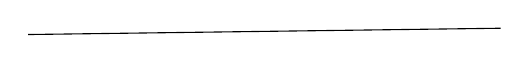
\begin{tikzpicture}\draw (0,0)--(6,0.08);\end{tikzpicture}}

17 Dold-Puppe, Whitehead etc

\figure{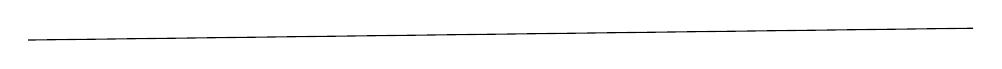
\begin{tikzpicture}\draw (0,0)--(12,.15);\end{tikzpicture}}
